\documentclass[]{article}
\usepackage{lmodern}
\usepackage{amssymb,amsmath}
\usepackage{ifxetex,ifluatex}
\usepackage{fixltx2e} % provides \textsubscript
\ifnum 0\ifxetex 1\fi\ifluatex 1\fi=0 % if pdftex
  \usepackage[T1]{fontenc}
  \usepackage[utf8]{inputenc}
\else % if luatex or xelatex
  \ifxetex
    \usepackage{mathspec}
  \else
    \usepackage{fontspec}
  \fi
  \defaultfontfeatures{Ligatures=TeX,Scale=MatchLowercase}
\fi
% use upquote if available, for straight quotes in verbatim environments
\IfFileExists{upquote.sty}{\usepackage{upquote}}{}
% use microtype if available
\IfFileExists{microtype.sty}{%
\usepackage{microtype}
\UseMicrotypeSet[protrusion]{basicmath} % disable protrusion for tt fonts
}{}
\usepackage[margin=2.54cm]{geometry}
\usepackage{hyperref}
\hypersetup{unicode=true,
            pdftitle={Assignment 3: Physical Properties of Rivers},
            pdfauthor={Theo Cai},
            pdfborder={0 0 0},
            breaklinks=true}
\urlstyle{same}  % don't use monospace font for urls
\usepackage{color}
\usepackage{fancyvrb}
\newcommand{\VerbBar}{|}
\newcommand{\VERB}{\Verb[commandchars=\\\{\}]}
\DefineVerbatimEnvironment{Highlighting}{Verbatim}{commandchars=\\\{\}}
% Add ',fontsize=\small' for more characters per line
\usepackage{framed}
\definecolor{shadecolor}{RGB}{248,248,248}
\newenvironment{Shaded}{\begin{snugshade}}{\end{snugshade}}
\newcommand{\AlertTok}[1]{\textcolor[rgb]{0.94,0.16,0.16}{#1}}
\newcommand{\AnnotationTok}[1]{\textcolor[rgb]{0.56,0.35,0.01}{\textbf{\textit{#1}}}}
\newcommand{\AttributeTok}[1]{\textcolor[rgb]{0.77,0.63,0.00}{#1}}
\newcommand{\BaseNTok}[1]{\textcolor[rgb]{0.00,0.00,0.81}{#1}}
\newcommand{\BuiltInTok}[1]{#1}
\newcommand{\CharTok}[1]{\textcolor[rgb]{0.31,0.60,0.02}{#1}}
\newcommand{\CommentTok}[1]{\textcolor[rgb]{0.56,0.35,0.01}{\textit{#1}}}
\newcommand{\CommentVarTok}[1]{\textcolor[rgb]{0.56,0.35,0.01}{\textbf{\textit{#1}}}}
\newcommand{\ConstantTok}[1]{\textcolor[rgb]{0.00,0.00,0.00}{#1}}
\newcommand{\ControlFlowTok}[1]{\textcolor[rgb]{0.13,0.29,0.53}{\textbf{#1}}}
\newcommand{\DataTypeTok}[1]{\textcolor[rgb]{0.13,0.29,0.53}{#1}}
\newcommand{\DecValTok}[1]{\textcolor[rgb]{0.00,0.00,0.81}{#1}}
\newcommand{\DocumentationTok}[1]{\textcolor[rgb]{0.56,0.35,0.01}{\textbf{\textit{#1}}}}
\newcommand{\ErrorTok}[1]{\textcolor[rgb]{0.64,0.00,0.00}{\textbf{#1}}}
\newcommand{\ExtensionTok}[1]{#1}
\newcommand{\FloatTok}[1]{\textcolor[rgb]{0.00,0.00,0.81}{#1}}
\newcommand{\FunctionTok}[1]{\textcolor[rgb]{0.00,0.00,0.00}{#1}}
\newcommand{\ImportTok}[1]{#1}
\newcommand{\InformationTok}[1]{\textcolor[rgb]{0.56,0.35,0.01}{\textbf{\textit{#1}}}}
\newcommand{\KeywordTok}[1]{\textcolor[rgb]{0.13,0.29,0.53}{\textbf{#1}}}
\newcommand{\NormalTok}[1]{#1}
\newcommand{\OperatorTok}[1]{\textcolor[rgb]{0.81,0.36,0.00}{\textbf{#1}}}
\newcommand{\OtherTok}[1]{\textcolor[rgb]{0.56,0.35,0.01}{#1}}
\newcommand{\PreprocessorTok}[1]{\textcolor[rgb]{0.56,0.35,0.01}{\textit{#1}}}
\newcommand{\RegionMarkerTok}[1]{#1}
\newcommand{\SpecialCharTok}[1]{\textcolor[rgb]{0.00,0.00,0.00}{#1}}
\newcommand{\SpecialStringTok}[1]{\textcolor[rgb]{0.31,0.60,0.02}{#1}}
\newcommand{\StringTok}[1]{\textcolor[rgb]{0.31,0.60,0.02}{#1}}
\newcommand{\VariableTok}[1]{\textcolor[rgb]{0.00,0.00,0.00}{#1}}
\newcommand{\VerbatimStringTok}[1]{\textcolor[rgb]{0.31,0.60,0.02}{#1}}
\newcommand{\WarningTok}[1]{\textcolor[rgb]{0.56,0.35,0.01}{\textbf{\textit{#1}}}}
\usepackage{graphicx,grffile}
\makeatletter
\def\maxwidth{\ifdim\Gin@nat@width>\linewidth\linewidth\else\Gin@nat@width\fi}
\def\maxheight{\ifdim\Gin@nat@height>\textheight\textheight\else\Gin@nat@height\fi}
\makeatother
% Scale images if necessary, so that they will not overflow the page
% margins by default, and it is still possible to overwrite the defaults
% using explicit options in \includegraphics[width, height, ...]{}
\setkeys{Gin}{width=\maxwidth,height=\maxheight,keepaspectratio}
\IfFileExists{parskip.sty}{%
\usepackage{parskip}
}{% else
\setlength{\parindent}{0pt}
\setlength{\parskip}{6pt plus 2pt minus 1pt}
}
\setlength{\emergencystretch}{3em}  % prevent overfull lines
\providecommand{\tightlist}{%
  \setlength{\itemsep}{0pt}\setlength{\parskip}{0pt}}
\setcounter{secnumdepth}{0}
% Redefines (sub)paragraphs to behave more like sections
\ifx\paragraph\undefined\else
\let\oldparagraph\paragraph
\renewcommand{\paragraph}[1]{\oldparagraph{#1}\mbox{}}
\fi
\ifx\subparagraph\undefined\else
\let\oldsubparagraph\subparagraph
\renewcommand{\subparagraph}[1]{\oldsubparagraph{#1}\mbox{}}
\fi

%%% Use protect on footnotes to avoid problems with footnotes in titles
\let\rmarkdownfootnote\footnote%
\def\footnote{\protect\rmarkdownfootnote}

%%% Change title format to be more compact
\usepackage{titling}

% Create subtitle command for use in maketitle
\providecommand{\subtitle}[1]{
  \posttitle{
    \begin{center}\large#1\end{center}
    }
}

\setlength{\droptitle}{-2em}

  \title{Assignment 3: Physical Properties of Rivers}
    \pretitle{\vspace{\droptitle}\centering\huge}
  \posttitle{\par}
    \author{Theo Cai}
    \preauthor{\centering\large\emph}
  \postauthor{\par}
    \date{}
    \predate{}\postdate{}
  

\begin{document}
\maketitle

\hypertarget{overview}{%
\subsection{OVERVIEW}\label{overview}}

This exercise accompanies the lessons in Hydrologic Data Analysis on the
physical properties of rivers.

\hypertarget{directions}{%
\subsection{Directions}\label{directions}}

\begin{enumerate}
\def\labelenumi{\arabic{enumi}.}
\tightlist
\item
  Change ``Student Name'' on line 3 (above) with your name.
\item
  Work through the steps, \textbf{creating code and output} that fulfill
  each instruction.
\item
  Be sure to \textbf{answer the questions} in this assignment document.
\item
  When you have completed the assignment, \textbf{Knit} the text and
  code into a single PDF file.
\item
  After Knitting, submit the completed exercise (PDF file) to the
  dropbox in Sakai. Add your last name into the file name (e.g.,
  ``Salk\_A03\_RiversPhysical.Rmd'') prior to submission.
\end{enumerate}

The completed exercise is due on 18 September 2019 at 9:00 am.

\hypertarget{setup}{%
\subsection{Setup}\label{setup}}

\begin{enumerate}
\def\labelenumi{\arabic{enumi}.}
\tightlist
\item
  Verify your working directory is set to the R project file,
\item
  Load the tidyverse, dataRetrieval, and cowplot packages
\item
  Set your ggplot theme (can be theme\_classic or something else)
\item
  Import a data frame called ``MysterySiteDischarge'' from USGS gage
  site 03431700. Upload all discharge data for the entire period of
  record. Rename columns 4 and 5 as ``Discharge'' and ``Approval.Code''.
  DO NOT LOOK UP WHERE THIS SITE IS LOCATED.
\item
  Build a ggplot of discharge over the entire period of record.
\end{enumerate}

\begin{Shaded}
\begin{Highlighting}[]
\CommentTok{#Session set up}
\KeywordTok{getwd}\NormalTok{()}
\end{Highlighting}
\end{Shaded}

\begin{verbatim}
## [1] "Z:/Hydrologic_Data_Analysis"
\end{verbatim}

\begin{Shaded}
\begin{Highlighting}[]
\KeywordTok{library}\NormalTok{(tidyverse)}
\end{Highlighting}
\end{Shaded}

\begin{verbatim}
## -- Attaching packages -------------------------------------------------------------------------------- tidyverse 1.2.1 --
\end{verbatim}

\begin{verbatim}
## v ggplot2 3.2.1     v purrr   0.3.2
## v tibble  2.1.3     v dplyr   0.8.3
## v tidyr   1.0.0     v stringr 1.4.0
## v readr   1.3.1     v forcats 0.4.0
\end{verbatim}

\begin{verbatim}
## -- Conflicts ----------------------------------------------------------------------------------- tidyverse_conflicts() --
## x dplyr::filter() masks stats::filter()
## x dplyr::lag()    masks stats::lag()
\end{verbatim}

\begin{Shaded}
\begin{Highlighting}[]
\KeywordTok{library}\NormalTok{(dataRetrieval)}
\KeywordTok{library}\NormalTok{(cowplot)}
\end{Highlighting}
\end{Shaded}

\begin{verbatim}
## 
## ********************************************************
\end{verbatim}

\begin{verbatim}
## Note: As of version 1.0.0, cowplot does not change the
\end{verbatim}

\begin{verbatim}
##   default ggplot2 theme anymore. To recover the previous
\end{verbatim}

\begin{verbatim}
##   behavior, execute:
##   theme_set(theme_cowplot())
\end{verbatim}

\begin{verbatim}
## ********************************************************
\end{verbatim}

\begin{Shaded}
\begin{Highlighting}[]
\KeywordTok{library}\NormalTok{(lubridate)}
\end{Highlighting}
\end{Shaded}

\begin{verbatim}
## 
## Attaching package: 'lubridate'
\end{verbatim}

\begin{verbatim}
## The following object is masked from 'package:cowplot':
## 
##     stamp
\end{verbatim}

\begin{verbatim}
## The following object is masked from 'package:base':
## 
##     date
\end{verbatim}

\begin{Shaded}
\begin{Highlighting}[]
\KeywordTok{theme_set}\NormalTok{(}\KeywordTok{theme_minimal_grid}\NormalTok{())}

\CommentTok{#Import dataset}
\NormalTok{MysterySiteDischarge <-}\StringTok{ }\KeywordTok{readNWISdv}\NormalTok{(}\DataTypeTok{siteNumbers =} \StringTok{"03431700"}\NormalTok{,}
                                  \DataTypeTok{parameterCd =} \StringTok{"00060"}\NormalTok{,}
                                  \DataTypeTok{startDate =} \StringTok{""}\NormalTok{,}
                                  \DataTypeTok{endDate =} \StringTok{""}\NormalTok{)}
\CommentTok{#Rename columns  }
\KeywordTok{names}\NormalTok{(MysterySiteDischarge)[}\DecValTok{4}\OperatorTok{:}\DecValTok{5}\NormalTok{] <-}\StringTok{ }\KeywordTok{c}\NormalTok{(}\StringTok{"Discharge"}\NormalTok{, }\StringTok{"Approval.Code"}\NormalTok{)}

\KeywordTok{attr}\NormalTok{(MysterySiteDischarge, }\StringTok{"variableInfo"}\NormalTok{)}
\end{Highlighting}
\end{Shaded}

\begin{verbatim}
##   variableCode           variableName              variableDescription
## 1        00060 Streamflow, ft&#179;/s Discharge, cubic feet per second
##       valueType  unit options noDataValue
## 1 Derived Value ft3/s    Mean          NA
\end{verbatim}

\begin{Shaded}
\begin{Highlighting}[]
\KeywordTok{attr}\NormalTok{(MysterySiteDischarge, }\StringTok{"siteInfo"}\NormalTok{)}
\end{Highlighting}
\end{Shaded}

\begin{verbatim}
##                                          station_nm  site_no agency_cd
## 1 RICHLAND CREEK AT CHARLOTTE AVE, AT NASHVILLE, TN 03431700      USGS
##   timeZoneOffset timeZoneAbbreviation dec_lat_va dec_lon_va       srs
## 1         -06:00                  CST   36.15122  -86.85427 EPSG:4326
##   siteTypeCd    hucCd stateCd countyCd network
## 1         ST 05130202      47    47037    NWIS
\end{verbatim}

\begin{Shaded}
\begin{Highlighting}[]
\CommentTok{#GGplot of entire period of record}
\NormalTok{MysteryPlot <-}
\StringTok{  }\KeywordTok{ggplot}\NormalTok{(MysterySiteDischarge, }\KeywordTok{aes}\NormalTok{(}\DataTypeTok{x =}\NormalTok{ Date, }\DataTypeTok{y =}\NormalTok{ Discharge)) }\OperatorTok{+}
\StringTok{  }\KeywordTok{geom_line}\NormalTok{() }\OperatorTok{+}
\StringTok{  }\KeywordTok{xlab}\NormalTok{(}\StringTok{"Year"}\NormalTok{)}
\KeywordTok{print}\NormalTok{(MysteryPlot)}
\end{Highlighting}
\end{Shaded}

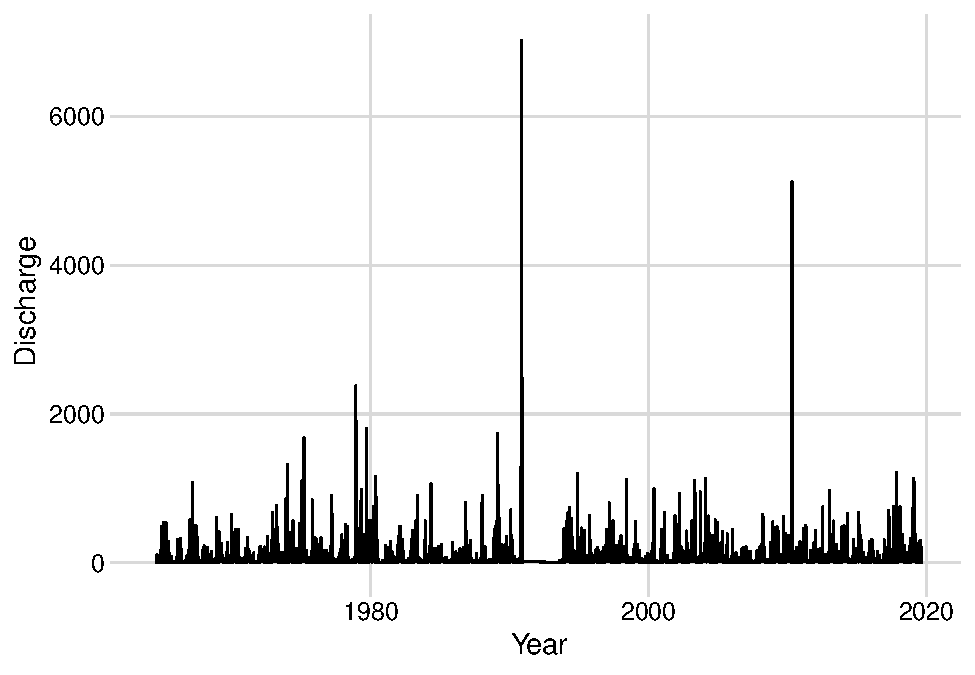
\includegraphics{Cai_A03_RiversPhysical_files/figure-latex/unnamed-chunk-1-1.pdf}

\hypertarget{analyze-seasonal-patterns-in-discharge}{%
\subsection{Analyze seasonal patterns in
discharge}\label{analyze-seasonal-patterns-in-discharge}}

\begin{enumerate}
\def\labelenumi{\arabic{enumi}.}
\setcounter{enumi}{4}
\tightlist
\item
  Add a ``Year'' and ``Day.of.Year'' column to the data frame.
\item
  Create a new data frame called ``MysterySiteDischarge.Pattern'' that
  has columns for Day.of.Year, median discharge for a given day of year,
  75th percentile discharge for a given day of year, and 25th percentile
  discharge for a given day of year. Hint: the summarise function
  includes \texttt{quantile}, wherein you must specify \texttt{probs} as
  a value between 0 and 1.
\item
  Create a plot of median, 75th quantile, and 25th quantile discharges
  against day of year. Median should be black, other lines should be
  gray.
\end{enumerate}

\begin{Shaded}
\begin{Highlighting}[]
\CommentTok{#Year column}
\NormalTok{MysterySiteDischarge <-}
\StringTok{  }\NormalTok{MysterySiteDischarge }\OperatorTok
\StringTok{  }\KeywordTok{mutate}\NormalTok{(}\DataTypeTok{Year =} \KeywordTok{year}\NormalTok{(Date))}
\CommentTok{#Day of Year column}
\NormalTok{MysterySiteDischarge <-}
\StringTok{  }\NormalTok{MysterySiteDischarge }\OperatorTok
\StringTok{  }\KeywordTok{mutate}\NormalTok{(}\DataTypeTok{Day.of.Year =} \KeywordTok{yday}\NormalTok{(Date))}

\CommentTok{#New Data Frame}
\NormalTok{MysterySiteDischarge.Pattern <-}
\StringTok{  }\NormalTok{MysterySiteDischarge }\OperatorTok
\StringTok{  }\KeywordTok{group_by}\NormalTok{(Day.of.Year) }\OperatorTok
\StringTok{  }\KeywordTok{summarise}\NormalTok{(}\DataTypeTok{MedianDischarge =} \KeywordTok{median}\NormalTok{(Discharge), }\DataTypeTok{SeventyFifthQ =} \KeywordTok{quantile}\NormalTok{(Discharge, }\DataTypeTok{probs =} \FloatTok{0.75}\NormalTok{), }
            \DataTypeTok{TwentyFifthQ =} \KeywordTok{quantile}\NormalTok{(Discharge, }\DataTypeTok{probs =} \FloatTok{0.25}\NormalTok{))}

\CommentTok{#Create GGplots}
\NormalTok{CombinedPlot <-}
\StringTok{  }\KeywordTok{ggplot}\NormalTok{(MysterySiteDischarge.Pattern, }\KeywordTok{aes}\NormalTok{(Day.of.Year)) }\OperatorTok{+}
\StringTok{  }\KeywordTok{geom_line}\NormalTok{(}\KeywordTok{aes}\NormalTok{(}\DataTypeTok{y =}\NormalTok{ MedianDischarge)) }\OperatorTok{+}
\StringTok{  }\KeywordTok{geom_line}\NormalTok{(}\KeywordTok{aes}\NormalTok{(}\DataTypeTok{y =}\NormalTok{ SeventyFifthQ), }\DataTypeTok{colour =} \StringTok{"808080"}\NormalTok{) }\OperatorTok{+}
\StringTok{  }\KeywordTok{geom_line}\NormalTok{(}\KeywordTok{aes}\NormalTok{(}\DataTypeTok{y =}\NormalTok{ TwentyFifthQ), }\DataTypeTok{colour =} \StringTok{"808080"}\NormalTok{) }\OperatorTok{+}
\StringTok{  }\KeywordTok{labs}\NormalTok{(}\DataTypeTok{x =} \StringTok{"Day of Year"}\NormalTok{, }\DataTypeTok{y =} \KeywordTok{expression}\NormalTok{(}\StringTok{"Discharge (ft"}\OperatorTok{^}\DecValTok{3}\OperatorTok{*}\StringTok{"/s)"}\NormalTok{))}
\KeywordTok{print}\NormalTok{(CombinedPlot)}
\end{Highlighting}
\end{Shaded}

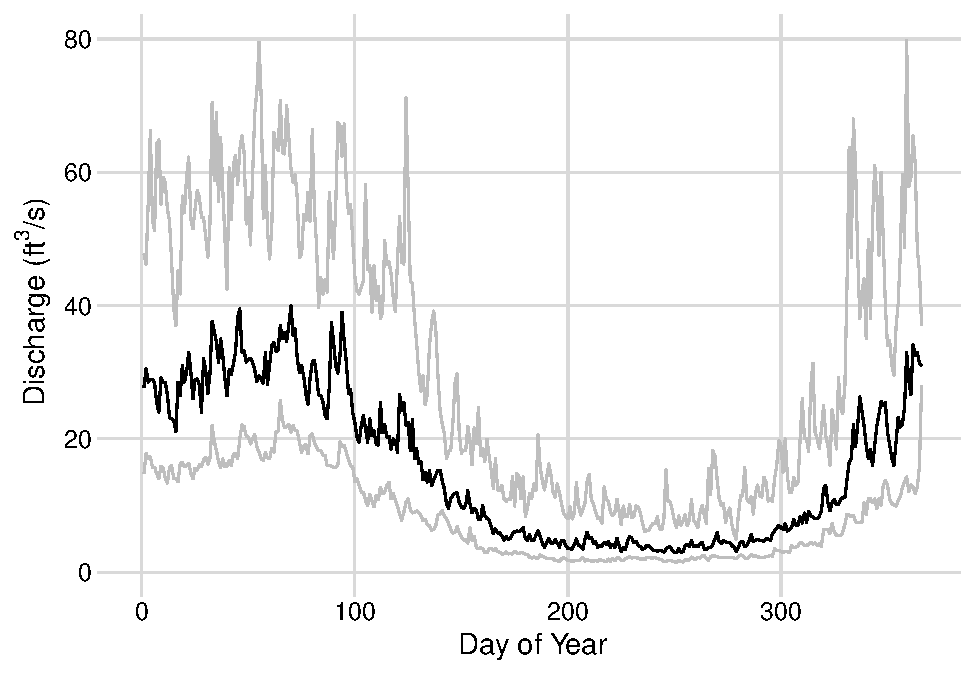
\includegraphics{Cai_A03_RiversPhysical_files/figure-latex/unnamed-chunk-2-1.pdf}

\begin{enumerate}
\def\labelenumi{\arabic{enumi}.}
\setcounter{enumi}{7}
\tightlist
\item
  What seasonal patterns do you see? What does this tell you about
  precipitation patterns and climate in the watershed?
\end{enumerate}

\begin{quote}
I see high discharge from November all the way till April/May. This
indicates to me that this location does not follow traditional temperate
patterns of weather, as it seems it experiences the most precipitation
in the winter months. I would guess that this watershed is in a hot
region that sees little rainfall in the summer but a lot in the winter -
as opposed to snow.
\end{quote}

\hypertarget{create-and-analyze-recurrence-intervals}{%
\subsection{Create and analyze recurrence
intervals}\label{create-and-analyze-recurrence-intervals}}

\begin{enumerate}
\def\labelenumi{\arabic{enumi}.}
\setcounter{enumi}{8}
\item
  Create two separate data frames for MysterySite.Annual.30yr (first 30
  years of record) and MysterySite.Annual.Full (all years of record).
  Use a pipe to create your new data frame(s) that includes the year,
  the peak discharge observed in that year, a ranking of peak
  discharges, the recurrence interval, and the exceedence probability.
\item
  Create a plot that displays the discharge vs.~recurrence interval
  relationship for the two separate data frames (one set of points
  includes the values computed from the first 30 years of the record and
  the other set of points includes the values computed for all years of
  the record.
\item
  Create a model to predict the discharge for a 100-year flood for both
  sets of recurrence intervals.
\end{enumerate}

\begin{Shaded}
\begin{Highlighting}[]
\CommentTok{#Make Date Frame}
\NormalTok{MysterySite.Annual}\FloatTok{.30}\NormalTok{yr <-}
\StringTok{  }\NormalTok{MysterySiteDischarge }\OperatorTok
\StringTok{  }\KeywordTok{filter}\NormalTok{(Year }\OperatorTok{<}\StringTok{ }\DecValTok{1994}\NormalTok{) }\OperatorTok
\StringTok{  }\KeywordTok{group_by}\NormalTok{(Year) }\OperatorTok
\StringTok{  }\KeywordTok{summarise}\NormalTok{(}\DataTypeTok{PeakDischarge =} \KeywordTok{max}\NormalTok{(Discharge)) }\OperatorTok
\StringTok{  }\KeywordTok{mutate}\NormalTok{(}\DataTypeTok{Rank =} \KeywordTok{rank}\NormalTok{(}\OperatorTok{-}\NormalTok{PeakDischarge),}
         \DataTypeTok{RecurrenceInterval =}\NormalTok{ (}\KeywordTok{length}\NormalTok{(Year) }\OperatorTok{+}\StringTok{ }\DecValTok{1}\NormalTok{)}\OperatorTok{/}\NormalTok{Rank,}
         \DataTypeTok{Probability =} \DecValTok{1}\OperatorTok{/}\NormalTok{RecurrenceInterval)}

\NormalTok{MysterySite.Annual.Full <-}
\StringTok{  }\NormalTok{MysterySiteDischarge }\OperatorTok
\StringTok{  }\KeywordTok{group_by}\NormalTok{(Year) }\OperatorTok
\StringTok{  }\KeywordTok{summarise}\NormalTok{(}\DataTypeTok{PeakDischarge =} \KeywordTok{max}\NormalTok{(Discharge)) }\OperatorTok
\StringTok{  }\KeywordTok{mutate}\NormalTok{(}\DataTypeTok{Rank =} \KeywordTok{rank}\NormalTok{(}\OperatorTok{-}\NormalTok{PeakDischarge),}
         \DataTypeTok{RecurrenceInterval =}\NormalTok{ (}\KeywordTok{length}\NormalTok{(Year) }\OperatorTok{+}\StringTok{ }\DecValTok{1}\NormalTok{)}\OperatorTok{/}\NormalTok{Rank,}
         \DataTypeTok{Probability =} \DecValTok{1}\OperatorTok{/}\NormalTok{RecurrenceInterval)}

\CommentTok{#Make plots}
\NormalTok{MysterySiteRecurrencePlot}\FloatTok{.30}\NormalTok{yr <-}
\StringTok{  }\KeywordTok{ggplot}\NormalTok{(MysterySite.Annual}\FloatTok{.30}\NormalTok{yr, }\KeywordTok{aes}\NormalTok{(}\DataTypeTok{x =}\NormalTok{ RecurrenceInterval, }\DataTypeTok{y =}\NormalTok{ PeakDischarge)) }\OperatorTok{+}
\StringTok{  }\KeywordTok{geom_point}\NormalTok{() }\OperatorTok{+}
\StringTok{  }\KeywordTok{labs}\NormalTok{(}\DataTypeTok{x =} \StringTok{"Recurrence Interval"}\NormalTok{, }\DataTypeTok{y =} \KeywordTok{expression}\NormalTok{(}\StringTok{"Discharge (ft"}\OperatorTok{^}\DecValTok{3}\OperatorTok{*}\StringTok{"/s)"}\NormalTok{))}
\KeywordTok{print}\NormalTok{(MysterySiteRecurrencePlot}\FloatTok{.30}\NormalTok{yr }\OperatorTok{+}\StringTok{ }\KeywordTok{ggtitle}\NormalTok{(}\StringTok{"First Thirty Years"}\NormalTok{))}
\end{Highlighting}
\end{Shaded}

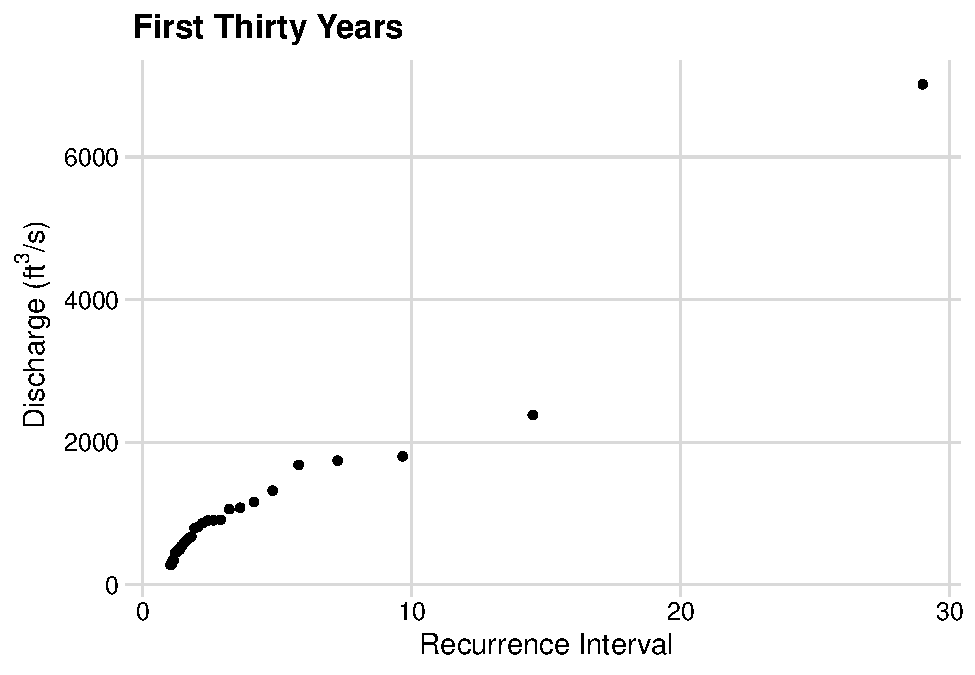
\includegraphics{Cai_A03_RiversPhysical_files/figure-latex/unnamed-chunk-3-1.pdf}

\begin{Shaded}
\begin{Highlighting}[]
\NormalTok{MysterySiteRecurrencePlot.Full <-}
\StringTok{  }\KeywordTok{ggplot}\NormalTok{(MysterySite.Annual.Full, }\KeywordTok{aes}\NormalTok{(}\DataTypeTok{x =}\NormalTok{ RecurrenceInterval, }\DataTypeTok{y =}\NormalTok{ PeakDischarge)) }\OperatorTok{+}
\StringTok{  }\KeywordTok{geom_point}\NormalTok{() }\OperatorTok{+}
\StringTok{  }\KeywordTok{labs}\NormalTok{(}\DataTypeTok{x =} \StringTok{"Recurrence Interval"}\NormalTok{, }\DataTypeTok{y =} \KeywordTok{expression}\NormalTok{(}\StringTok{"Discharge (ft"}\OperatorTok{^}\DecValTok{3}\OperatorTok{*}\StringTok{"/s)"}\NormalTok{))}
\KeywordTok{print}\NormalTok{(MysterySiteRecurrencePlot.Full }\OperatorTok{+}\StringTok{ }\KeywordTok{ggtitle}\NormalTok{(}\StringTok{"Full Time Period"}\NormalTok{))}
\end{Highlighting}
\end{Shaded}

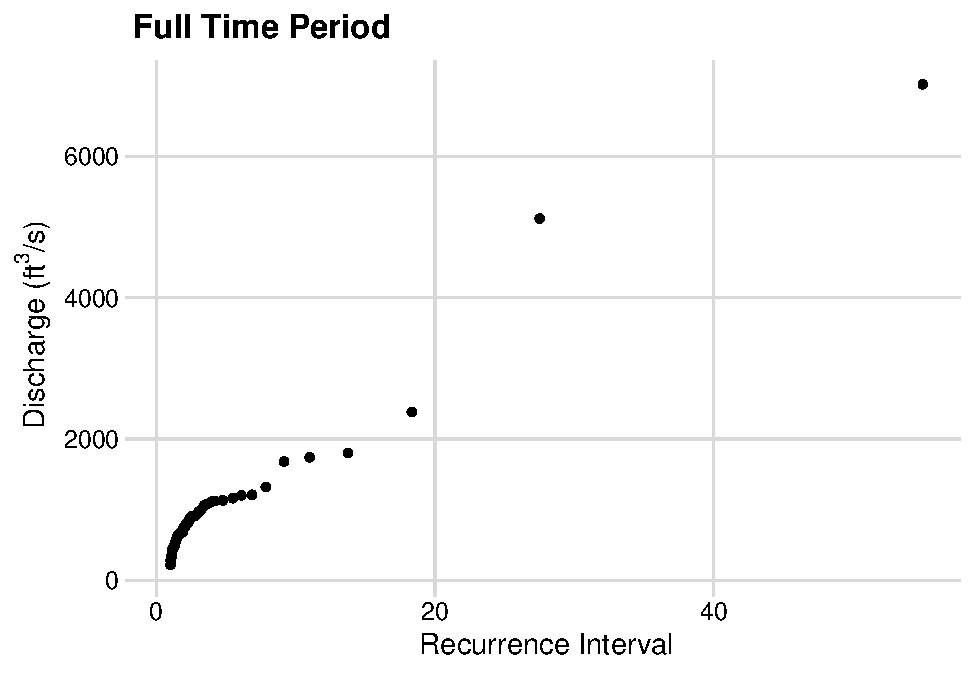
\includegraphics{Cai_A03_RiversPhysical_files/figure-latex/unnamed-chunk-3-2.pdf}

\begin{Shaded}
\begin{Highlighting}[]
\CommentTok{#Recurrence Models}
\NormalTok{Mystery}\FloatTok{.30}\NormalTok{yr.RImodel <-}\StringTok{ }\KeywordTok{lm}\NormalTok{(}\DataTypeTok{data =}\NormalTok{ MysterySite.Annual}\FloatTok{.30}\NormalTok{yr, PeakDischarge }\OperatorTok{~}\StringTok{ }\KeywordTok{log}\NormalTok{(RecurrenceInterval))}
\KeywordTok{summary}\NormalTok{(Mystery}\FloatTok{.30}\NormalTok{yr.RImodel)}
\end{Highlighting}
\end{Shaded}

\begin{verbatim}
## 
## Call:
## lm(formula = PeakDischarge ~ log(RecurrenceInterval), data = MysterySite.Annual.30yr)
## 
## Residuals:
##     Min      1Q  Median      3Q     Max 
## -982.36 -366.95   42.38  247.09 2838.21 
## 
## Coefficients:
##                         Estimate Std. Error t value Pr(>|t|)    
## (Intercept)               -107.5      197.3  -0.545     0.59    
## log(RecurrenceInterval)   1273.8      157.1   8.107 1.38e-08 ***
## ---
## Signif. codes:  0 '***' 0.001 '**' 0.01 '*' 0.05 '.' 0.1 ' ' 1
## 
## Residual standard error: 689.4 on 26 degrees of freedom
## Multiple R-squared:  0.7166, Adjusted R-squared:  0.7057 
## F-statistic: 65.73 on 1 and 26 DF,  p-value: 1.377e-08
\end{verbatim}

\begin{Shaded}
\begin{Highlighting}[]
\NormalTok{Mystery.Full.RImodel <-}\StringTok{ }\KeywordTok{lm}\NormalTok{(}\DataTypeTok{data =}\NormalTok{ MysterySite.Annual.Full, PeakDischarge }\OperatorTok{~}\StringTok{ }\KeywordTok{log}\NormalTok{(RecurrenceInterval))}
\KeywordTok{summary}\NormalTok{(Mystery.Full.RImodel)}
\end{Highlighting}
\end{Shaded}

\begin{verbatim}
## 
## Call:
## lm(formula = PeakDischarge ~ log(RecurrenceInterval), data = MysterySite.Annual.Full)
## 
## Residuals:
##     Min      1Q  Median      3Q     Max 
## -955.95 -236.29   41.91  210.67 2805.35 
## 
## Coefficients:
##                         Estimate Std. Error t value Pr(>|t|)    
## (Intercept)               -2.001    116.322  -0.017    0.986    
## log(RecurrenceInterval) 1052.234     88.834  11.845   <2e-16 ***
## ---
## Signif. codes:  0 '***' 0.001 '**' 0.01 '*' 0.05 '.' 0.1 ' ' 1
## 
## Residual standard error: 578.3 on 52 degrees of freedom
## Multiple R-squared:  0.7296, Adjusted R-squared:  0.7244 
## F-statistic: 140.3 on 1 and 52 DF,  p-value: < 2.2e-16
\end{verbatim}

\begin{Shaded}
\begin{Highlighting}[]
\CommentTok{#100-Year Recurrence}
\NormalTok{Mystery}\FloatTok{.30}\NormalTok{yr.RImodel}\OperatorTok{$}\NormalTok{coefficients[}\DecValTok{1}\NormalTok{] }\OperatorTok{+}\StringTok{ }\NormalTok{Mystery}\FloatTok{.30}\NormalTok{yr.RImodel}\OperatorTok{$}\NormalTok{coefficients[}\DecValTok{2}\NormalTok{]}\OperatorTok{*}\KeywordTok{log}\NormalTok{(}\DecValTok{100}\NormalTok{)}
\end{Highlighting}
\end{Shaded}

\begin{verbatim}
## (Intercept) 
##    5758.621
\end{verbatim}

\begin{Shaded}
\begin{Highlighting}[]
\NormalTok{Mystery.Full.RImodel}\OperatorTok{$}\NormalTok{coefficients[}\DecValTok{1}\NormalTok{] }\OperatorTok{+}\StringTok{ }\NormalTok{Mystery.Full.RImodel}\OperatorTok{$}\NormalTok{coefficients[}\DecValTok{2}\NormalTok{]}\OperatorTok{*}\KeywordTok{log}\NormalTok{(}\DecValTok{100}\NormalTok{)}
\end{Highlighting}
\end{Shaded}

\begin{verbatim}
## (Intercept) 
##    4843.717
\end{verbatim}

\begin{enumerate}
\def\labelenumi{\arabic{enumi}.}
\setcounter{enumi}{11}
\tightlist
\item
  How did the recurrence interval plots and predictions of a 100-year
  flood differ among the two data frames? What does this tell you about
  the stationarity of discharge in this river?
\end{enumerate}

\begin{quote}
The recurrence interval plot of the first thirty years of data
definitely shows us that, historically, the curve of the recurrence log
was less extreme. The slope of the increase of discharge per increase in
recurrence interval used to be smaller than that of the full time
period. Curiously, however, the 100-year flood discharge for the past is
greater than that of the full period. This tells me that the
stationarity of discharge in this river is fairly stable - perhaps there
have been minor changes to the system, but in general there doesn't seem
to have been any major landscape or environmental changes throughout the
entire time period.
\end{quote}

\hypertarget{reflection}{%
\subsection{Reflection}\label{reflection}}

\begin{enumerate}
\def\labelenumi{\arabic{enumi}.}
\setcounter{enumi}{12}
\tightlist
\item
  What are 2-3 conclusions or summary points about river discharge you
  learned through your analysis?
\end{enumerate}

\begin{quote}
I found that river discharge isn't always as cut and dry as ``snow melt
in spring = high discharge around same time.'' Additionally, I found
that it was possible for the discharge of 100-Year floods to decrease
from the past to the present, indicating that either global warming
isn't affecting certain sites as much as others, or that it is affecting
different sites differently depending on geographical location.
\end{quote}

\begin{enumerate}
\def\labelenumi{\arabic{enumi}.}
\setcounter{enumi}{13}
\tightlist
\item
  What data, visualizations, and/or models supported your conclusions
  from 13?
\end{enumerate}

\begin{quote}
CombinedPlot helped me realize conclusion \#1, while all of the
Recurrence plots/models helped me realize conclusion \#2.
\end{quote}

\begin{enumerate}
\def\labelenumi{\arabic{enumi}.}
\setcounter{enumi}{14}
\tightlist
\item
  Did hands-on data analysis impact your learning about discharge
  relative to a theory-based lesson? If so, how?
\end{enumerate}

\begin{quote}
Yes, it did! It forced me to organize and extrapolate the information
for myself, rather than just giving it to me. It taught me to read and
recognize patterns of a larger theory.
\end{quote}

\begin{enumerate}
\def\labelenumi{\arabic{enumi}.}
\setcounter{enumi}{15}
\tightlist
\item
  How did the real-world data compare with your expectations from
  theory?
\end{enumerate}

\begin{quote}
The real-world data matched up a little bit. I didn't expect the site to
be in Tennessee, but I guess I at least got right the fact that it's
technically in the South.
\end{quote}


\end{document}
